\documentclass[journal,12pt,twocolumn]{IEEEtran}
%
\usepackage{setspace}
\usepackage{gensymb}
\usepackage{siunitx}
\usepackage{tkz-euclide} 
\usepackage{textcomp}
\usepackage{standalone}
\usetikzlibrary{calc}
\newcommand\hmmax{0}
\newcommand\bmmax{0}

%\doublespacing
\singlespacing

%\usepackage{graphicx}
%\usepackage{amssymb}
%\usepackage{relsize}
\usepackage[cmex10]{amsmath}
%\usepackage{amsthm}
%\interdisplaylinepenalty=2500
%\savesymbol{iint}
%\usepackage{txfonts}
%\restoresymbol{TXF}{iint}
%\usepackage{wasysym}
\usepackage{amsthm}
%\usepackage{iithtlc}
\usepackage{mathrsfs}
\usepackage{txfonts}
\usepackage{stfloats}
\usepackage{bm}
\usepackage{cite}
\usepackage{cases}
\usepackage{subfig}
%\usepackage{xtab}
\usepackage{longtable}
\usepackage{multirow}
%\usepackage{algorithm}
%\usepackage{algpseudocode}
\usepackage{enumitem}
\usepackage{mathtools}
\usepackage{steinmetz}
\usepackage{tikz}
\usepackage{circuitikz}
\usepackage{verbatim}
\usepackage{tfrupee}
\usepackage[breaklinks=true]{hyperref}
%\usepackage{stmaryrd}
\usepackage{tkz-euclide} % loads  TikZ and tkz-base
%\usetkzobj{all}
\usetikzlibrary{calc,math}
\usepackage{listings}
    \usepackage{color}                                            %%
    \usepackage{array}                                            %%
    \usepackage{longtable}                                        %%
    \usepackage{calc}                                             %%
    \usepackage{multirow}                                         %%
    \usepackage{hhline}                                           %%
    \usepackage{ifthen}                                           %%
  %optionally (for landscape tables embedded in another document): %%
    \usepackage{lscape}     
\usepackage{multicol}
\usepackage{chngcntr}
\usepackage{amsmath}
\usepackage{cleveref}
\usepackage{amsmath}
%\usepackage{enumerate}

%\usepackage{wasysym}
%\newcounter{MYtempeqncnt}
\DeclareMathOperator*{\Res}{Res}
%\renewcommand{\baselinestretch}{2}
\renewcommand\thesection{\arabic{section}}
\renewcommand\thesubsection{\thesection.\arabic{subsection}}
\renewcommand\thesubsubsection{\thesubsection.\arabic{subsubsection}}

\renewcommand\thesectiondis{\arabic{section}}
\renewcommand\thesubsectiondis{\thesectiondis.\arabic{subsection}}
\renewcommand\thesubsubsectiondis{\thesubsectiondis.\arabic{subsubsection}}

% correct bad hyphenation here
\hyphenation{op-tical net-works semi-conduc-tor}
\def\inputGnumericTable{}                                 %%

\lstset{
%language=C,
frame=single, 
breaklines=true,
columns=fullflexible
}
%\lstset{
%language=tex,
%frame=single, 
%breaklines=true
%}
\usepackage{graphicx}
\usepackage{pgfplots}

\begin{document}


\newtheorem{theorem}{Theorem}[section]
\newtheorem{problem}{Problem}
\newtheorem{proposition}{Proposition}[section]
\newtheorem{lemma}{Lemma}[section]
\newtheorem{corollary}[theorem]{Corollary}
\newtheorem{example}{Example}[section]
\newtheorem{definition}[problem]{Definition}
%\newtheorem{thm}{Theorem}[section] 
%\newtheorem{defn}[thm]{Definition}
%\newtheorem{algorithm}{Algorithm}[section]
%\newtheorem{cor}{Corollary}
\newcommand{\BEQA}{\begin{eqnarray}}
\newcommand{\EEQA}{\end{eqnarray}}
\newcommand{\define}{\stackrel{\triangle}{=}}
\bibliographystyle{IEEEtran}
%\bibliographystyle{ieeetr}
\providecommand{\mbf}{\mathbf}
\providecommand{\abs}[1]{\ensuremath{\left\vert#1\right\vert}}
\providecommand{\norm}[1]{\ensuremath{\left\lVert#1\right\rVert}}
\providecommand{\mean}[1]{\ensuremath{E\left[ #1 \right]}}
\providecommand{\pr}[1]{\ensuremath{\Pr\left(#1\right)}}
\providecommand{\qfunc}[1]{\ensuremath{Q\left(#1\right)}}
\providecommand{\sbrak}[1]{\ensuremath{{}\left[#1\right]}}
\providecommand{\lsbrak}[1]{\ensuremath{{}\left[#1\right.}}
\providecommand{\rsbrak}[1]{\ensuremath{{}\left.#1\right]}}
\providecommand{\brak}[1]{\ensuremath{\left(#1\right)}}
\providecommand{\lbrak}[1]{\ensuremath{\left(#1\right.}}
\providecommand{\rbrak}[1]{\ensuremath{\left.#1\right)}}
\providecommand{\cbrak}[1]{\ensuremath{\left\{#1\right\}}}
\providecommand{\lcbrak}[1]{\ensuremath{\left\{#1\right.}}
\providecommand{\rcbrak}[1]{\ensuremath{\left.#1\right\}}}
\theoremstyle{remark}
\newtheorem{rem}{Remark}
\newcommand{\sgn}{\mathop{\mathrm{sgn}}}
\providecommand{\res}[1]{\Res\displaylimits_{#1}} 
%\providecommand{\norm}[1]{\lVert#1\rVert}
\providecommand{\mtx}[1]{\mathbf{#1}}
\providecommand{\fourier}{\overset{\mathcal{F}}{ \rightleftharpoons}}
%\providecommand{\hilbert}{\overset{\mathcal{H}}{ \rightleftharpoons}}
\providecommand{\system}{\overset{\mathcal{H}}{ \longleftrightarrow}}
	%\newcommand{\solution}[2]{\textbf{Solution:}{#1}}
\newcommand{\solution}{\noindent \textbf{Solution: }}
\newcommand{\cosec}{\,\text{cosec}\,}
\providecommand{\dec}[2]{\ensuremath{\overset{#1}{\underset{#2}{\gtrless}}}}
\newcommand{\myvec}[1]{\ensuremath{\begin{pmatrix}#1\end{pmatrix}}}
\newcommand{\mydet}[1]{\ensuremath{\begin{vmatrix}#1\end{vmatrix}}}
%\numberwithin{equation}{section}
\numberwithin{equation}{subsection}
%\numberwithin{problem}{section}
%\numberwithin{definition}{section}
\makeatletter
\@addtoreset{figure}{problem}
\makeatother
\let\StandardTheFigure\thefigure
\let\vec\mathbf
%\renewcommand{\thefigure}{\theproblem.\arabic{figure}}
\renewcommand{\thefigure}{\theproblem}
%\setlist[enumerate,1]{before=\renewcommand\theequation{\theenumi.\arabic{equation}}
%\counterwithin{equation}{enumi}
%\renewcommand{\theequation}{\arabic{subsection}.\arabic{equation}}
\def\putbox#1#2#3{\makebox[0in][l]{\makebox[#1][l]{}\raisebox{\baselineskip}[0in][0in]{\raisebox{#2}[0in][0in]{#3}}}}
     \def\rightbox#1{\makebox[0in][r]{#1}}
     \def\centbox#1{\makebox[0in]{#1}}
     \def\topbox#1{\raisebox{-\baselineskip}[0in][0in]{#1}}
\vspace{3cm}
\title{Equivalent Kernel}
\maketitle
\newpage
%\tableofcontents
\bigskip
\renewcommand{\thefigure}{\theenumi}
\renewcommand{\thetable}{\theenumi}
\begin{abstract}
This document contains theory involved in curve fitting.
\end{abstract}
\section{\textbf{Objective}}
The objective is to use an equivalent kernel on a noisy data.
\section{Generate Dataset}
Create a sinusoidal function of the form
\begin{align}
    y = A\sin{2\pi x} + n(t) \label{eq:1}
\end{align}
n(t) is the random noise that is included in the training set. This set consists of N samples of input data i.e. x expressed as shown below
\begin{align}
    x = \myvec{x_{1}, x_{2}, .., x_{N}}^{T}
\end{align}
which give the corresponding values of y denoted as
\begin{align}
    y = \myvec{y_{1}, y_{2}, .., y_{N}}^{T}
\end{align}

The corresponding values of y are generated from the Eq \eqref{eq:1}.The first term $A\sin{2\pi x}$ is computed directly and then random noise samples having a normal(Gaussian) distribution are added inorder to get the corresponding values of y.
\begin{lstlisting}
#Generate the sine curve 
noise = 0.5
A = 2  
# Noisy training data
X_train = np.arange(-3, 4, 1).reshape(-1, 1)
Y_train = A*np.sin(2*np.pi*X_train) + noise * np.random.randn(*X_train.shape)
\end{lstlisting}

The generated input matrix would look like
\begin{align}
    \vec{F}= \myvec{ 1 & x_{0} & x_{0}^2 & \ldots & x_{0}^{N-1} \\
		1 & x_{1} & x_{1}^2 & \ldots & x_{1}^{N-1} \\
		1 & x_{2} & x_{2}^2 & \ldots & x_{2}^{N-1} \\
		\vdots & & \vdots &  & \vdots  \\
		    1 & \ldots & \ldots & \ldots & x_{N}^{N-1} }\label{eq:12}
\end{align}
\section{Polynomial Curve Fitting}
The goal is to find the best line that fits into the  pattern of the training data shown in the graph.
We shall fit the data using a polynomial function of the form, 
\begin{align}
     y\brak{w,x}= \sum_{j=0}^{M} w_j x^{j}\\
\end{align}
M is the order of the polynomial
The polynomial coefficient are collectively denoted by the vector $\vec{w}$.The proposed vector $\vec{w}$ of the model referring to Eq \eqref{eq:12} is given by 
\begin{align}
    \hat{\vec{w}} = \brak{\vec{F}^T\vec{F}}^{-1}\vec{F}^Ty \label{eq:13}
\end{align}

\section{Equivalent Kernel}
For Bayesian treatment of linear regression, we introduce a prior probability distribution over the model parameters $\vec{w}$.

The corresponding conjugate prior is therefore given by a Gaussian
distribution of the form
\begin{align}
    p(\vec{w}) = N(\vec{w} | \vec{m_{0}},\vec{S_{0}})
\end{align}
having mean $\vec{m_{0}}$ and covariance $\vec{S_{0}}$.

We now compute the posterior distribution, which is proportional to the product of the likelihood function and the prior which takes the form
\begin{align}
    p(\vec{w} | t) = N(\vec{w} | \vec{m_{N}},\vec{S_{N}}) \label{eq : posterior}
\end{align}
Since the prior is Gaussian, so would be the posterior.
In Eq \eqref{eq : posterior},
\begin{align}
       \vec{m}_{N} = \vec{S}_{N}\brak{\vec{S}_{0}^{-1}\vec{m}_{0} + \beta \vec{f}^T \vec{t}}\\
       \vec{S}_{N}^{-1} = \vec{S}_{0}^{-1} + \beta \vec{f}^{T} \vec{f}
\end{align}
Specifically, we consider a zero - mean isotropic Gaussian governed by a single precision parameter $\alpha$ so that
\begin{align}
    p(\vec{w} | \alpha) = N(\vec{w} | 0, \alpha^{-1} \vec{I})
\end{align}
Then the corresponding posterior distribution over $\vec{w}$ is then given as
\begin{align}
    \vec{m}_{N} = \beta\vec{S}_{N} \vec{f}^T \vec{t} \label{eq : mean}\\
    \vec{S}_{N}^{-1} = \alpha \vec{I} + \beta \vec{f}^{T} \vec{f}
\end{align}
The predictive mean can be written in the form
\begin{multline}
     y(\vec{x},\vec{m}_{N}) = \vec{m}_{N} f(x)\\
        = \beta f(\vec{x})^{T} S_{N} \vec{f}^{T} \vec{t} \\
        = \sum_{n=1}^{N} \beta f(\vec{x})^{T} S_{N} f(\vec{x}_{n}) t_{n}
\end{multline}
The mean of the predictive distribution at a point $\vec{x}$ is given by a linear combination of the training set target variables $t_{n}$ , so
\begin{align}
    y(\vec{x},\vec{m}_{N}) = \sum_{n=1}^{N} k(\vec{x},\vec{x}^{'}) t_{n}
\end{align}
where
\begin{align}
    k(\vec{x},\vec{x}_{n}) = \beta f(\vec{x})^{T} S_{N} f(\vec{x}^{'}) \label{eq : kernel}
\end{align}
Eq \eqref{eq : kernel} is known as the smoother matrix of the equivalent kernel.

Further insight into the role of the equivalent kernel can be obtained by considering the covariance between $y(\vec{x})$ and $y(\vec{x}^{'})$ given by
\begin{align}
    cov[y(\vec{x}),y(\vec{x}^{'})] = cov[f(\vec{x})^{T}\vec{w}, \vec{w}^{T}f(\vec{x}^{'})]\\
         = f(\vec{x})^{T} S_{N} f(\vec{x}^{'})\\
         = \beta^{-1}k(\vec{x},\vec{x}^{'})
\end{align}
we define a localized kernel directly and use this to make predictions for new input vectors $\vec{x}$.

This leads to practical frameworks for regression known as Gaussian Processes.

An effective kernel should satisfy
\begin{align}
    \sum_{n=1}^{N} k(\vec{x},\vec{x}_{n}) = 1
\end{align}
for all values of x.

Eq \eqref{eq : kernel} satisfies the general equation of kernel, that can be expressed in the form an inner product with respect to a vector $f(\vec{x})$ of non linear functions given by
\begin{align}
      k(\vec{x},\vec{z}) = \psi(\vec{x})^{T}\psi(\vec{z})
\end{align}
where
\begin{align}
    \psi(\vec{x}) = \beta^{\frac{1}{2}}S_{N}^{\frac{1}{2}} f(\vec{x})
\end{align}
\section{Implementation using numPy}
Here, we will use the squared exponential kernel, also known as Gaussian kernel.
given by 
\begin{align}
    k(\vec{x}_{i},\vec{x}_{j}) = \sigma_{f}^{2} \exp{-\frac{1}{2l^2}(\vec{x}_i - \vec{x}_j)^{T}(\vec{x}_{i} - \vec{x}_{j})} \label{eq : kernel_1}
\end{align}
The length $l$ controls the smoothness of the function and $\sigma_{f}$ the vertical variation

We define the kernel Eq \eqref{eq : kernel_1},
\begin{lstlisting}
#Kernel 
def kernel(X1, X2, l=1.0, sigma_f=1.0):
    sqdist = np.sum(X1**2, 1).reshape(-1, 1) + np.sum(X2**2, 1) - 2 * np.dot(X1, X2.T)
    return sigma_f**2 * np.exp(-0.5 / l**2 * sqdist)
\end{lstlisting}
We use a function for plotting the samples
\begin{lstlisting}
 def plot_gp(mu, cov, X, X_train=None, Y_train=None, samples=[]):
    X = X.ravel()
    mu = mu.ravel()
    uncertainty = 1.96 * np.sqrt(np.diag(cov))
    
    plt.fill_between(X, mu + uncertainty, mu - uncertainty, alpha=0.1)
    plt.plot(X, mu, label='Mean')
    for i, sample in enumerate(samples):
        plt.plot(X, sample, lw=1, ls='--', label=f'Sample {i+1}')
    if X_train is not None:
        plt.plot(X_train, Y_train, 'rx')
    plt.legend()
\end{lstlisting}
The following code draws three random samples and plots it together with the zero mean.
\begin{lstlisting}
import numpy as np
import matplotlib.pyplot as plt

X = np.arange(-5, 5, 0.2).reshape(-1, 1)

mu = np.zeros(X.shape)
cov = kernel(X, X)

# Draw three samples from the prior
samples = np.random.multivariate_normal(mu.ravel(), cov, 3)

# Plot GP mean, confidence interval and samples 
plot_gp(mu, cov, X, samples=samples)
\end{lstlisting}
The Plot would look as below shown in Fig \ref{fig:2} 
\begin{figure}[!h]
\begin{center}
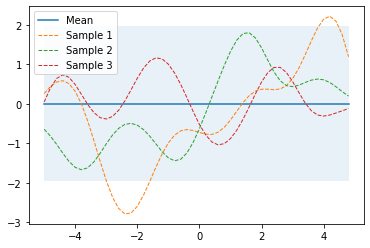
\includegraphics[width=3.4in]{figs/fig2.png}
\end{center}
\caption{}
\label{fig:2}
\end{figure}

We define the posterior as
\begin{lstlisting}
from numpy.linalg import inv

def posterior(X_s, X_train, Y_train, l=1.0, sigma_f=1.0, sigma_y=1e-8):
    K = kernel(X_train, X_train, l, sigma_f) + sigma_y**2 * np.eye(len(X_train))
    K_s = kernel(X_train, X_s, l, sigma_f)
    K_ss = kernel(X_s, X_s, l, sigma_f) + 1e-8 * np.eye(len(X_s))
    K_inv = inv(K)
    
    # Equation (7)
    mu_s = K_s.T.dot(K_inv).dot(Y_train)

    # Equation (8)
    cov_s = K_ss - K_s.T.dot(K_inv).dot(K_s)
    
    return mu_s, cov_s
\end{lstlisting}
Now , the prediction from noisy training data
\begin{lstlisting}
noise = 0.5
A = 2  
# Noisy training data
X_train = np.arange(-3, 4, 1).reshape(-1, 1)
Y_train = A*np.sin(2*np.pi*X_train) + noise * np.random.randn(*X_train.shape)

# Compute mean and covariance of the posterior distribution
mu_s, cov_s = posterior(X, X_train, Y_train, sigma_y=noise)

samples = np.random.multivariate_normal(mu_s.ravel(), cov_s, 3)
plot_gp(mu_s, cov_s, X, X_train=X_train, Y_train=Y_train, samples=samples)
\end{lstlisting}
Th plot would look like in Fig \ref{fig:1}
\begin{figure}[!h]
\begin{center}
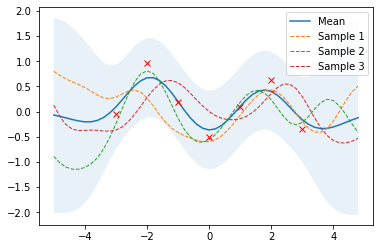
\includegraphics[width=3.4in]{figs/fig1.png}
\end{center}
\caption{}
\label{fig:1}
\end{figure}

Python code:
\begin{lstlisting}
https://github.com/Hrithikraj2/EE4015_IDP/blob/main/Assignment_6/Assignment_6.ipynb
\end{lstlisting}
\end{document}
